\documentclass[a4paper]{article}

\usepackage{INTERSPEECH2018}
\usepackage{booktabs}
\usepackage{adjustbox}
\usepackage{multirow}
\usepackage{textcomp}
\usepackage{caption}
\usepackage{subcaption}

\title{Multilingual Multi-Task Learning for Low-Resource Acoustic Modeling}

\name{Josh Meyer$^1$}
%The maximum number of authors in the author list is twenty. If the number of contributing authors is more than twenty, they should be listed in a footnote or in acknowledgement section, as appropriate.
\address{
  $^1$University of Arizona}
\email{joshua.richard.meyer@gmail.com}

\begin{document}

\maketitle
% 
\begin{abstract}
  
\end{abstract}
\noindent\textbf{Index Terms}: speech recognition, multi-task learning, acoustic modeling





\section{Introduction}

Previous work has shown that performance for a low-resource language on speech recognition can be improved by adding training data from another, resource-rich language. Typically, data from another language is added as a separate task in the Multi-Task Learning framework  \cite{caruana1997} via an additional output layer. The targets for this addititional language have typically been states of context-dependent triphones, defined by some tree clustering algorithm.

This current research builds off the intuition that triphones encode information which is too fine-grained to be maximally useful for language-transfer. Using a higher-level of linguistic abstraction (eg. the monophone), we are able to better extract the kind of language-general information useful in training an acoustic model for some target language.

The intuition being that when adding a source language as an auxialilary task, it would be better to focus on source-language distinctions which are robust and will transfer well to a new, target language.

Each auxiliary task is created by redefining the parameters of the HMM-GMM system used to bootstrap the DNN-hybrid system, such that the phonetic decision tree is cut short.

The target language is Kyrgyz, and the source language is English. Both data come from audiobooks, English being from LibriSpeech and Kyrgyz from the Bizdin.kg project.




\section{Background}


The earliest examples of MTL with multiple languages can be found in \cite{huang2013} and \cite{heigold2013}, who both used triphones from each language as additional tasks. They were interested in improving performance on all languages, not just one target language. These two studies were then followed up in multiple other threads of research. More recently, \cite{grezl2016} found that adding more triphones from a single, well-resourced language (English) actually leads to better performance, but this could be conflated with the fact that they did not use any weighting scheme, and as such, the source language with fewer states and more data would more quickly overfit, leaving less of a chance for the target language to exert influence during backprop.


In another direction, multiple works have investigated MTL for a single language, without any source language transfer. These approaches aim to find tasks which are phonetically relevant to the main task. Both \cite{seltzer2013} and later \cite{huang2015} looked at a very similar approach to what I explore here, with MTL on broader, more abstract phonetic categories for English. They both found improvement on TIMIT, but they didn't investigate multi-lingual transfer. With regards to low-resource languages, \cite{chen2014} and later \cite{chen2015} similarly looked at MTL for a single target language, using graphemes or a universal phoneset as extra targets.



\section{DNN-Hybrid Training as Model Transfer}

The standard DNN-Hybrid approach requires the GMM-HMM system to provide the labels for supervised training. This reliance of the DNN on GMM alignments is actually a form of model transfer, where the DNN is trained to perform the extact same classification as its GMM predecessor. The DNN not only learns the frame alignments from the individual GMMs, but also the DNN indirectly learns the structure of the phonetic decision tree used to define the tied-state system. This is because the output layer of the DNN is trained to predict targets which were defined via leaves of the decision tree, as is shown in Figure (\ref{fig:tree-net})\footnote{The graphic for the decision tree comes from \cite{young2002} and the neural net graphic comes from \cite{heigold2013}}.


\begin{figure}[!htbp]
  \centering
\minipage{0.5\textwidth}
  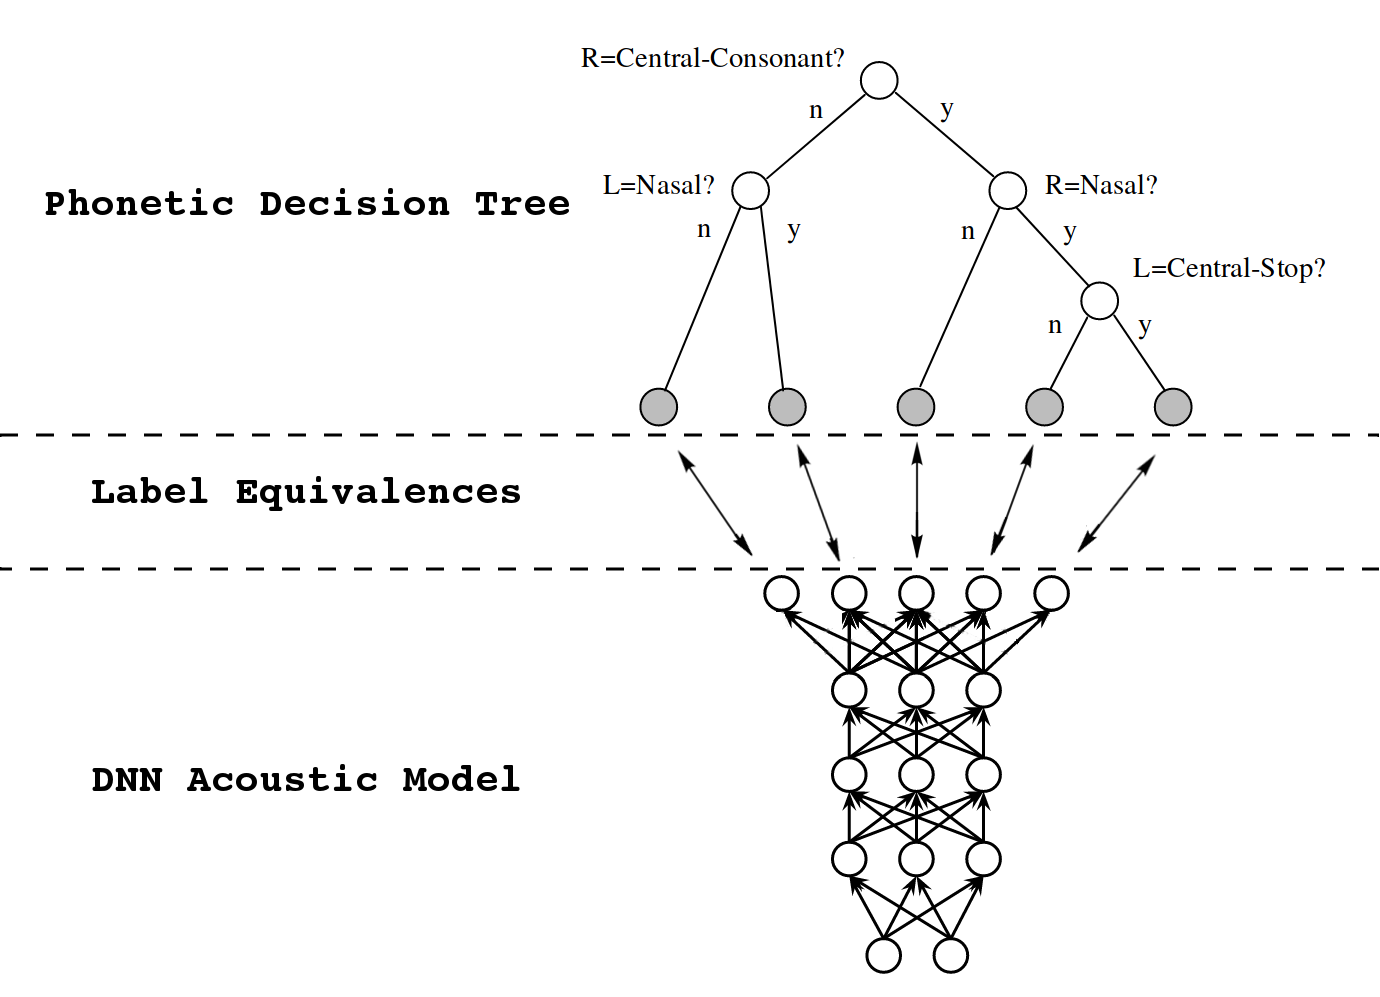
\includegraphics[width=\linewidth]{figs/tree-net.png}
  \caption{GMM$\rightarrow$DNN Model Transfer}
    \label{fig:tree-net}
  \endminipage\hfill
\end{figure}


Given that standard triphones encode very fine-grained information which may not help performance on a target language, the following experiments investigate GMM$\rightarrow$DNN model transfer at a higher level for an additional source language. 


\section{Experiments}

This work investigates the application of MTL technique to low resource acoustic modeling. All experiments simulate a common development scenario: there exists little transcribed data for the target language, but lots of data in some source language.

The following experiments tease out (1) the level of detail at which the source language should be modeled and (2) the amount of weighting which should be given to the target language training examples.

The first point of interest is the level of detail at which the source language is modeled. This is investigated via addition of multiple tasks to the TDNN during training. The experiements here are crafted to answer the question: \textit{how much phonetic detail should the source language be modeled at to best transfer data to the target language?}.

We can model the source language with lots of contextual detail (ie. the triphone), with abstracted, context-independent detail (ie. the monophone), or somewhere in between. Building of the traditional hybrid DNN-HMM ASR training pipeline, investigating these levels of representation are easily acheived via the phonetic decision tree. We can merely assign labels to training data frames by moving up the tree, from leaves (triphones) to roots (monophones).

The second point of interest is the relative weighting of target vs. source language training data. It is clear that if we train two languages in parallel, the source language (with many more training samples) will dominate the target language in the fight for influence during backprop.

To my knowledge this has not been investigated in ASR acoustic modeling, although it was dedicated its own chapter in Caruana's 1997 dissertation. To investigate weighting further, I examine the following target vs. source weighting schemes: 1-to-2, 1-to-1, and 2-to-1 (all ratios are target-to-source).

These weights are instantiated during training via a weight to the target output label, where the label is a one-hot vector. For example, given 1000 hours of source language and 1 hour of target language, to acheive a 1-to-1 ratio in training, I would multiply the target labels from the target language by 1000, resulting in target vectors such as \texttt{$[0, 0, 0, 0, 1000, 0, 0, \ldots]$} instead of \texttt{$[0, 0, 0, 0, 1, 0, 0, \ldots]$}. The final layer is a ReLU activation, so having a target value higher than $1$ is not an issue as it would be with a traditional softmax layer.



\subsection{Data}

Two speech corpora are used in the following experiments:

\begin{enumerate}
\item $\approx$ 5 hours of LibriSpeech (4.86 hours)
\item $\approx$ 1.5 hours of Kyrgyz audiobook (1.59 hours)
\end{enumerate}

\subsection{Model Building}

All models were build using the Kaldi \texttt{nnet3} approach. The main neural net run script used in this paper can be found at www.github.com/JRMeyer/kaldi-mirror/egs/kgz/kyrgyz-model/run\_nnet3\_multilingual.sh. The main GMM script used to create data alignments can be found at www.github.com/JRMeyer/kaldi-mirror/egs/kgz/kyrgyz-model/run\_gmm.sh.

\subsubsection{Decision Trees}

In GMM training, monophones (for each language) were allotted 1,000 Gaussian components, and trained over 25 iterations of EM. These monophones were then expanded into context-dependent triphones via a phonetic decision tree, with a maximum of 2,000 leaves \& 5,000 Gaussians (LibriSpeech reached 1584 leaves, and Kyrgyz reached 752). The resulting tied-state clusters (ie. leaves) are then trained as context-dedendent triphones over 25 iterations of EM.


\subsubsection{Multi-Task Neural Net Acoustic Models}

Given the alignments from the GMM-HMM models, a 5-layer, 500-dimensional TDNN is trained over 10 epochs of backprop on a single GPU instance.

Each auxiliary task is implemented as a separate output layer along with a separate, penultimate hidden layer. All other hidden layers of the TDNN are trained in parallel.

During testing, \textit{only} the main task is used. The additional tasks are dropped and the baseline Kyrgyz triphones are used in decoding. This highlights the purpose of the extra tasks: to force the learning of robust representations in the hidden layers during training. The tasks may in fact not be the best option for final classification; they serve as ``training wheels'' which are then removed once the net is ready.



\textbf{Baseline Model}

All the following architectures will be compared to the performance of a baseline model of identical architecture (5 hidden layers, 500-dimentional layers, ReLU activations, same training algorithm). The output targets are standard context-dependent triphones trained on Kyrgyz audio.

To account for any advantage mutliple output layers may bring about, the baseline contains two output layers, where the tasks are identical. In this way, random initializations in the weights and biases for each task are accounted for.

\textbf{Auxiliary Tasks}

The auxiliary tasks all train on English language data from the LibriSpeech corpus. Investigating the intuition that labels generated by a standard triphone phonetic decision tree are not the best representation of data for transfer learning, the auxiliary tasks here investigate different levels in the decision tree's branches.

I split the LibriSpeech phonetic decision tree into three logical parts, shown in Figure (\ref{fig:tree-parts}):

\begin{enumerate}
\item roots (standard monophones)
\item branches (what I dub, ``half''-phones)
\item leaves (standard triphones)
\end{enumerate}




\begin{figure}[!htbp]
  \centering
\minipage{0.525\textwidth}
  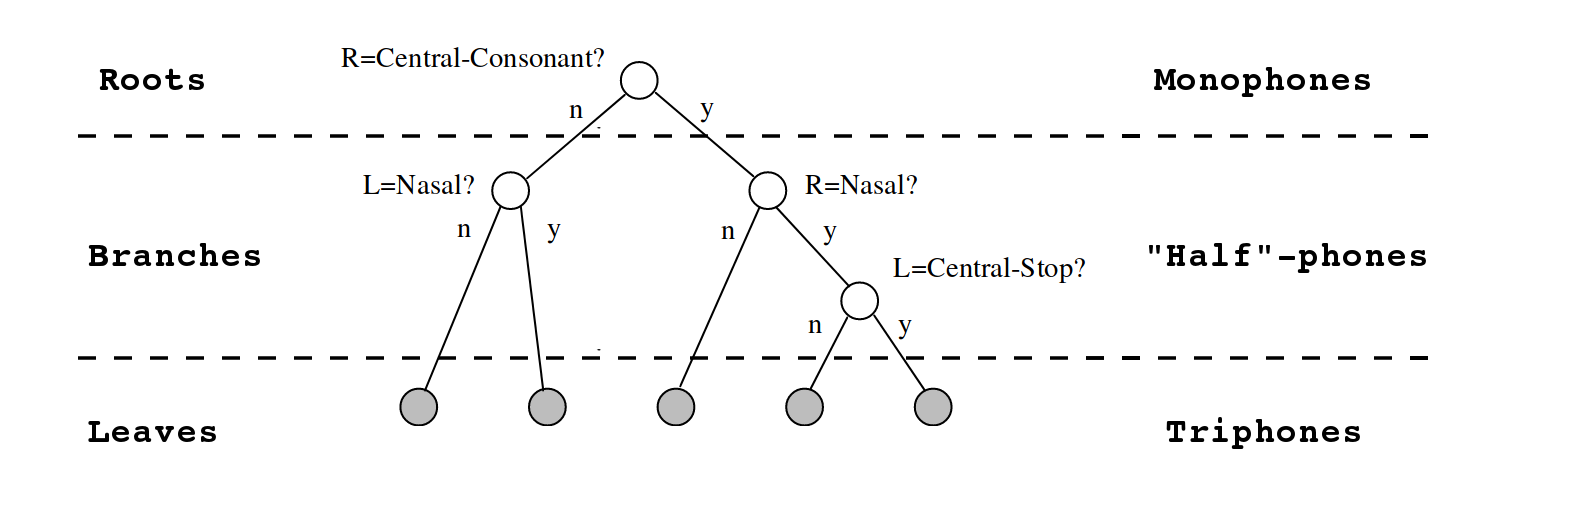
\includegraphics[width=\linewidth]{figs/levels.png}
  \caption{Logical Tree Parts}
  \label{fig:tree-parts}
\endminipage\hfill
\end{figure}


The ``half''-phones were created by halving the optimal number of leaves from the triphone system (ie. 1584 leaves) and re-training a new GMM-HMM system with half the optimal number of leaves (1/2 * 1584 = 792 leaves). All the other parameters were left unchanged (number of Gaussian components, iterations of EM, etc.). An overview of the auxiliary tasks can be found in Table (\ref{tab:tasks}).




\begin{table}[!htbp]
  \centering
  \caption{Auxiliary Tasks}
  \label{tab:tasks}
  \begin{adjustbox}{width=.45\textwidth}
    \begin{tabular}{lcc}
      \toprule
      \textbf{Logical Tree Part} & \textbf{Level of Phonetic Detail} & \textbf{ \textnumero~of Tasks}\\
      \midrule
      Roots & Monophones & 1\\
      Branches & Half-phones & 1\\
      Leaves & Triphones & 1\\ 
      Lower Tree & Monophones + Half-phones & 2\\
      Upper Tree & Half-phones + Triphones & 2\\
      Whole Tree & Monophones + Half-phones + Triphones & 3\\
      \bottomrule
    \end{tabular}
  \end{adjustbox}
\end{table}

Each of the above tasks were trained on the 5 hour section of LibriSpeech corpus. They are included as an extra output layer in the TDNN.


By forcing the neural net to recognize higher levels in the tree, we will learn representations which are more abstract, and therefore more likely to be relevant multi-lingually. 


The addition of each above task adds approximately 5 hours of training data to the standard training of a Single Task Model on Kyrgyz. As such, a weighting procedure was used to balance the relative influence of source vs. target training data on backprop. For example, to reach a one-to-one ratio, where one hour of Kyrgyz is equal to one hour of English, I multiplied every Kyrgyz target one-hot vector by $3.06$. The exact weighting scheme is shown in Table (\ref{tab:weights}).

\begin{table}[!htbp]
  \centering
  \caption{Target:Source Data Weighting Scheme}
  \label{tab:weights}
  \begin{adjustbox}{width=.3\textwidth}
    \begin{tabular}{cc}
      \toprule
      \textbf{Target:Source Ratio} & \textbf{Target Weight}\\
      \midrule
      1:2 & 1.53x  \\
      1:1 & 3.06x  \\
      2:1 & 6.12x  \\
      \bottomrule
    \end{tabular}
  \end{adjustbox}
\end{table}




\subsection{Results}


All results are performed on the same held-out section of Kyrgyz audiobook. The bigram language model, lexicon, and main-task decision tree are built into a standard decoding graph in the traditional Kaldi style. Decoding is performed with a bigram backoff language model trained on a Wikipedia Kyrgyz dump, and contains, 103,998 unigrams and 56,6871 bigrams.


\begin{enumerate}
\item Any amount of English beats out Kyrgyz-only baseline.
\item Triphones work better than monophones (except for the 2-to-1 weighting).
\item Both languages / tasks overfit (referencing frame-classification logs)
\item atai overfit slower with additional tasks
\item atai overfits with monophones earlier, I think because it's an easier task
\item only train on 30 minutes of Krygyz... more likely to find an effect
\end{enumerate}


Below in Table (\ref{tab:results}) are the Word Error Rates relative to the baseline, single-task model. They all show improvement over the baseline. However, the result that triphones work best is not new, and my ``half''-phones don't beat them out strictly speaking.

I do see a trend with the +1 extra tasks: the more I increase the ratio of target-to-source data, the better abstract tasks perform. That is, the more data I have in the target language, the better it is to model the source language higher in the tree.

None of the +2 or +3 tasks outperform the more simple, +1 tasks. I would have hoped that modeling the whole tree at all levels would perform best, but that isn't the case.


\begin{table}[!htbp]
  \centering
  \caption{Word Error Rates (WER\%) Relative to Baseline}
    \label{tab:results}
  \begin{adjustbox}{width=.45\textwidth}
    \begin{tabular}{lccc}
      \toprule
      & \multicolumn{3}{c}{\textbf{Target:Source Weighting}} \\
      \textbf{Auxiliary (Source Lang) Tasks} & \textit{1-to-2} & \textit{1-to-1} & \textit{2-to-1}\\
      \midrule
      STL Baseline                          &  \multicolumn{3}{c}{50.54\% WER}  \\
      Monophones                            &  -3.13  & -3.22 & \textbf{-2.34}  \\
      Halfphones                            &  -1.86  & \textbf{-3.81} & -1.86 \\
      Triphones                             &  \textbf{-3.81} & -3.42 & -1.17  \\
      Monophones + Halfphones               &  -2.44  & -2.05 &  \textbf{-2.34}\\
      Halfphones + Triphones                &  -2.64  & -2.54 & -0.49 \\
      Monophones + Halfphones + Halfphones  &  -1.95  & -2.34 &  -1.66\\
      \midrule
      AVERAGE                               &  -2.64  & -2.90 & -1.64 \\
      \bottomrule
    \end{tabular}
  \end{adjustbox}
\end{table}


%% \begin{table}[!htbp]
%%   \centering
%%     \caption{TDNN // 5-layer // 500-dim //  10 epoch }
%%   \begin{adjustbox}{width=.45\textwidth}
%%     \begin{tabular}{lccc}
%%       \toprule
%%       & \multicolumn{3}{c}{\textbf{Target:Source Weighting}} \\
%%       \textbf{Auxiliary (Source Lang) Tasks} & \textit{1-to-2} & \textit{1-to-1} & \textit{2-to-1}\\
%%       \midrule
%%       STL Baseline                          &  \multicolumn{3}{c}{50.54}  \\
%%       Monophones                            &  47.41  & 47.32 & 48.20  \\
%%       Halfphones                            &  48.68  & 46.73 & 48.68 \\
%%       Triphones                             &  46.73  & 47.12 & 49.37  \\
%%       Monophones + Halfphones               &  48.10  & 48.49 & 48.20 \\
%%       Halfphones + Triphones                &  47.90  & 48.00 & 50.05\\
%%       Monophones + Halfphones + Halfphones  &  48.59  & 48.20 & 48.88\\
%%       \bottomrule
%%     \end{tabular}
%%     \label{table:data}
%%   \end{adjustbox}
%% \end{table}





\section{Discussion}

We can draw a few conclusions from these results. One result, which few researcher discuss, is that Multi-Task Learning is not guaranteed to yeild better results. In my experiments on language transfer from English $\rightarrow$ Kyrgyz via MTL, I found that more than one task led to reduced performance (compared to just one extra task). However, every MTL model beat out the STL baseline.

Another, more interesting take-away is that the exists an interaction between level of detail in the target task and target vs. source data weighting. Looking just at the MTL experiments with one extra task (monophones OR halfphones OR triphones), we see a trend. The more weight we give to the target data, the less detail we want in the source task (to produce better results).

Thinking about the reasons this trend may exist, we think about the relationship between tasks, their learning patterns, and their influence on shared hidden layers.

A task with fewer labels is typically easier to learn, finds a local minimum more quickly, and is less willing to budge once it is settled.

This behavior results in simple source tasks (with more weighting relative to target) pulling the hidden layers more than target. So if we have a MTL net with two tasks, if the source task is easy, and there's a lot of data for it, the target task won't be able to exert enough influence during backprop to find good hidden weights for itself.

A source task which is more complicated (ie. more labels) will take longer to learn, and as such, the target task will be able to exert more influence on the shared hidden layers.


Looking at Figure (\ref{fig:1-to-2}), we see the models' performance during training on (1) training data or (2) held-out validation data, we find some support for this explanation.


\begin{figure}[!htbp]
\centering
\begin{subfigure}{.25\textwidth}
  \centering
  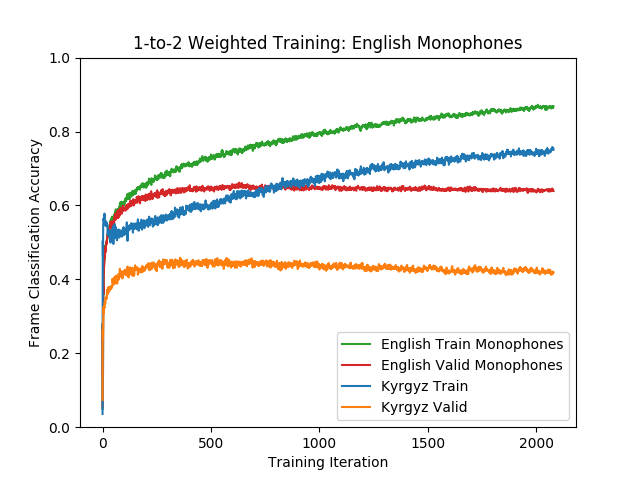
\includegraphics[width=1.1\textwidth,keepaspectratio]{figs/1-to-2-mono.png}
  \caption{Aux Task = Monophones}
  \label{fig:sub1}
\end{subfigure}%
\begin{subfigure}{.25\textwidth}
  \centering
  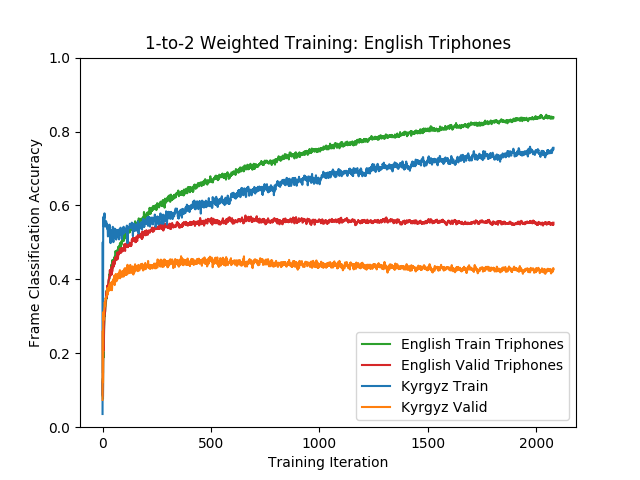
\includegraphics[width=1.1\textwidth,keepaspectratio]{figs/1-to-2-tri.png}
  \caption{Aux Task = Triphones}
  \label{fig:sub2}
\end{subfigure}
\caption{1-to-2 Weighted MTL Training | Kyrgyz and English Classification Accuracy}
\label{fig:1-to-2}
\end{figure}


Firstly, let's compare two models which were trained with the same 1-to-2 (target-to-source) weighting scheme, but different levels of abstraction (ie. monophones vs triphones). We see that the performance on English training data (in Green) is better than performance on Kyrgyz training data (in Blue). This is the case for the monophone model and triphone model. Also we see that the model generalizes better for English than for Kyrgyz (ie. English validation (Red) is better than Kyrgyz validation (Orange)).

In general, out of all these measures, our aim is to increase the Kyrgyz validation performance (Orange). We can take away from these graphs a few things. Firstly, looking at the performance on English, the triphone model performs worse than the monophone model. That is, at the end of 10 epochs, performance on monophone train and validation data is higher than on triphone train and validation data. Both models clearly overfit, with validation performance plateauing after about 500 iterations, but monophone classification reaches over 60\% accuracy vs. under 60\% accuracy for triphones. This makes sense, because the model has around 1500 labels for train and only around 200 for monophones.




Taking a look at the 2-to-1 weighting scheme in Figure (\ref{fig:2-to-1}), where the Kyrgyz data has more importance during backprop, we see a very different picture.


\begin{figure}[!htbp]
\centering
\begin{subfigure}{.25\textwidth}
  \centering
  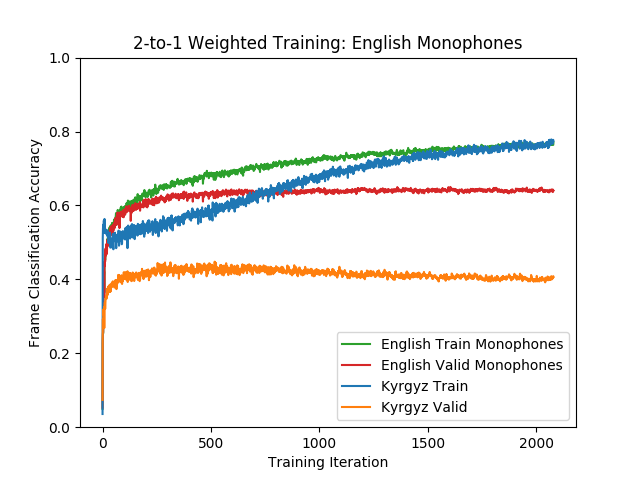
\includegraphics[width=1.1\textwidth,keepaspectratio]{figs/2-to-1-mono.png}
  \caption{Aux Task = Monophones}
  \label{fig:sub1}
\end{subfigure}%
\begin{subfigure}{.25\textwidth}
  \centering
  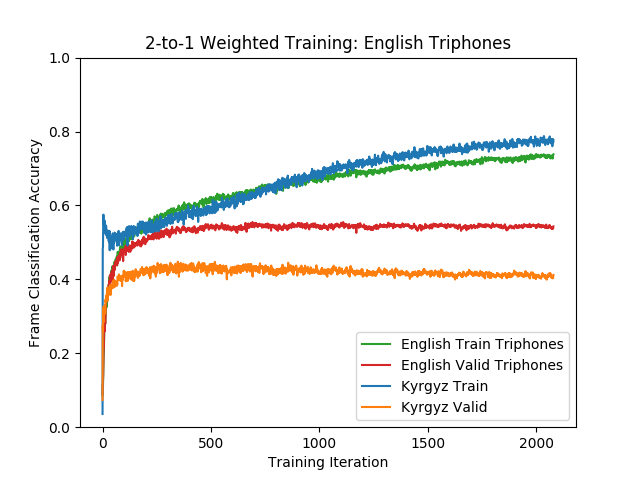
\includegraphics[width=1.1\textwidth,keepaspectratio]{figs/2-to-1-tri.png}
  \caption{Aux Task = Triphones}
  \label{fig:sub2}
\end{subfigure}
\caption{2-to-1 Weighted MTL Training | Kyrgyz and English Classification Accuracy}
\label{fig:2-to-1}
\end{figure}


We can see that even though the Kyrgyz data is more heavily weighted, the English monophones quickly overfit. However, the shared hidden layers clearly favor the Kyrgyz data, and the model fits to Kyrgyz more rapidly than it does to English. The weight eventually overfit to both models equally.

Looking over at the performance of the model trained with English triphones as an auxiliary task, we find that not the model fits the Kyrgyz training data, but by the end of 2000 iterations (10 epochs), the weights have found a local minimum which is better for Kyrgyz than English. The influence of the English triphones during backprop is too diffuse to steer the hidden layer weights in direction favorable to the auxiliary task, English.


\section{Conclusions}

Multi-Task Learning promises a very simple solution to a very hard problem. It would seem that as long as we can add relevant tasks to our net, through the good graces of backprop, a best solution will automatically be discovered. It would also seem that we are guaranteed to get better results as long as we keep adding related tasks. This study shows that the picture is not so simple.

Starting with three additional tasks, which are clearly related \textit{a priori}, the current study investigated not only their relative import, but also the dynamics of their combinations. Each task represented a level of abstraction from the typical training labels, from fine-grained (triphones), to more abstract (half-phones) to completely context-free (monophones). In addition to these three levels (deduced from a given decision tree), I tested logical combinations of abstractions: the entire tree, the top half of the tree, and the bottom half of the tree. None of these combinations outperformed the tasks added individually.

Discussed more deeply than the results of combinations of tasks was the performance of the tasks with regards to differential weighting and their level of abstraction. Their level of abstraction correlates to number of labels in the task, and as such number of nodes in the output layer, and as such number of parameters in the model. With more labels, the task is inherently more difficult and the model has more parameters to train. As such, models with fewer labels found their local minimum more quickly, and were less likely to succeed influence over shared hidden layers to another task (ie. Kyrgyz).

If a task is simple, the net will find a good local minimum quickly. As such, in MTL setups, care should be taken to weighting auxiliary tasks relative to their simplicity.

Hard tasks exert less of an influence on other tasks, but simple tasks can dominate during training. As such, care must be taken to weight accordingly, even if tasks are related.




\section{Acknowledgements}

I'd like to thank Dan Povey for answering my (oftentimes naive) questions on the kaldi-help Google Group.

I'd like to also thank Chorobek Saadanbekov and Murat Jumashev for making the Kyrgyz audiobook available to me through the Bizdin.kg group.

This material is based upon work supported by the National Science Foundation Graduate Research Fellowship under Grant No. (DGE-1746060). Any opinion, findings, and conclusions or recommendations expressed in this material are those of the authors(s) and do not necessarily reflect the views of the National Science Foundation.

\newpage

\bibliographystyle{IEEEtran}
\bibliography{mybib}



\end{document}
